\section{Software di basso livello per invio dati}

La scheda ESP32 è stata programmata da Arduino: non sono state utilizzate librerie (a parte ovviamente \mcode{Wire.h}), ma ci si è rifatti a \cite{MPU6050_tockn} e \cite{MPU9250} come riferimento per la costruzione del programma.\\
Di seguito una breve panoramica del funzionamento.

\subsection{Setup}

Il programma inizia facendo un check di tutti i canali del multiplexer e inizializzando le IMU presenti.\\
Poiché i giroscopi potrebbero misurare angoli diversi da 0 all'avvio, è stata implementata la possibilità di calibrarli tramite la funzione \mcode{calc_gyro_offset()}, che richiede di lasciare l'IMU immobile per raccogliere misure di velocità angolari di cui poi verrà fatta la media, che sarà il bias che viene poi sottratto a ogni successiva lettura; questa funzione è attivabile e disattivabile tramite la variabile booleana \mcode{calibrate_gyro}.\\

Durante il setup viene mandato un segnale al magnetometro con la funzione \mcode{initAK8963()}, e se l'IMU in questione è una 9250 ad esso segue l'inizializzazione del magnetometro, mentre se è una 6050 si interrompe senza fare nulla.\\
Per le MPU-9250 è stata anche implementata la possibilità di calibrare i magnetometri tramite la funzione \mcode{calc_magn_hard_iron_soft_iron_offset()} per eliminare i bias soft-iron, dati da interferenze di materiali magnetici, e hard-iron, date da parti che generano un proprio campo magnetico presenti sulla scheda stessa (basti pensare al campo magnetico prodotto dalla corrente che scorre in un circuito); questa funzione è attivabile e disattivabile tramite la variabile booleana \mcode{calibrate_magn}.\\
Riferimenti sulla calibrazione del magnetometro in \cite{MPU9250}, \cite{ozyagcilar2012calibrating} e \cite{ozyagcilar2012implementing}.\\

\begin{figure}[H]
    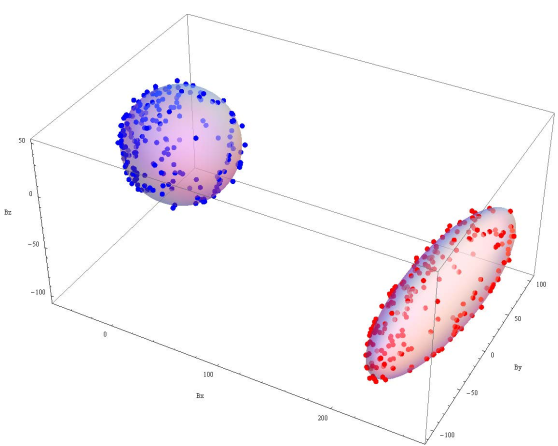
\includegraphics[scale=0.65]{immagini/distorsione campo magnetico confronto.PNG}
    \centering
    \caption{Campo magnetico corretto (sferico e centrato in $\overline{0}$) a sinistra, a confronto con campo magnetico distorto (bias hard-iron lo decentrano e bias sof-iron lo deformano) a destra.}
\end{figure}

Un'ultima funzione, normalmente disattivata, \mcode{I2C_scan()}, permette di effettuare uno scan di tutti i possibili address sul canale I2C per controllare quali dispositivi rispondono per ogni canale del multiplexer: tale funzione è stata particolarmente utile nelle fasi di sviluppo e debugging del progetto.\\

\subsection{Lettura dati}

Nel loop principale i dati vengono letti e stampati su seriale a ogni iterazione.\\

La funzione \mcode{read_data()} (che richiama la sotto-funzione \mcode{read_raw_data()}) consente di accedere ai registri di memoria delle IMU e ricostruire la giusta lettura, prima unendo i byte raw (high e low), e poi correggendo con apposite variabili date su datasheet o con le misure di bias trovate se sono state effettuate calibrazioni nella fase di setup.\\

La lettura dei dati delle IMU avviene a una frequenza di 400 kHz complessivi e quindi ogni IMU viene letta a circa 130 kHz. Ogni dato da leggere è composto da 8 bit e sono presenti 9 misure da leggere, conseguentemente 72 bit per ogni MPU.\\
La velocità del canale I2C risulta sufficiente per avere un buon aggiornamento della stima e un delay ridotto.\\


La funzione \mcode{print_data()} invece invia al seriale i dati letti, in modo che possano essere recepiti da PC ed elaborati nel filtro.


\clearpage